\begin{titlepage}
    \centering
    \vspace{1cm}

    \textbf{\LARGE Generative Models for Boundary Representations}

    \vspace{1.5cm}

    \textbf{Sebastian Lochmann} \\
    Matriculation Number: 20-925-020

    \vspace{0.5cm}

    \textit{Thesis Supervisors:} \\
    Matthew Keeler, IDEAL lab \\
    Dr. Daniel Wälchli, Manukai AG \\

    \vfill

    In Fulfillment of the Requirements\\
    for the Degree of \\
    Master of Science ETH in Computational Science and Engineering

    \vfill

    % Begin minipage environment for logos
    \begin{minipage}{0.32\textwidth}
        \centering
        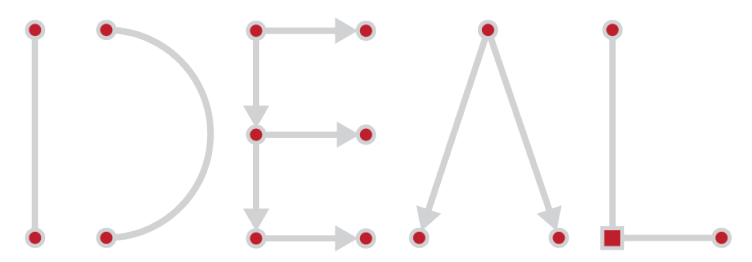
\includegraphics[width=0.6\textwidth]{figures/IDEAL_logo_25.png}
    \end{minipage}%
    \hfill
    \begin{minipage}{0.32\textwidth}
        \centering
        
\includegraphics[width=\textwidth]{figures/eth_logo.pdf}
    \end{minipage}
    \hfill
    \begin{minipage}{0.32\textwidth}
        \centering
        
\includegraphics[width=\textwidth]{figures/manukai_logo.png}
    \end{minipage}
    % End minipage environment

    \vspace{0.5cm}

    \textbf{Swiss Federal Institute of Technology Zurich}\\
    Department of Mechanical and Process Engineering (D-MAVT) \\
    IDEAL – Chair of Artificial Intelligence in Engineering Design \\
    Manukai AG - ETH-Spinoff for AI Manufacturing

    \vspace{1cm}

    \textbf{March 2026}

    Spring Semester 2026

\end{titlepage}
